\documentclass[main.tex]{subfiles}
\begin{document}


\section{Symmetries}\label{ch18}

В классических и в квантовых системах мы имеем теорему Нётер [16, 63]:
Всякий раз, когда в системе существует непрерывная симметрия, существует связанная с ней консервативная величина.
Примерами являются сохранение импульса (симметрия трансляции), сохранение энергии (симметрия относительно трансляций времени) и угловой момент (симметрия вращения). В классических системах теорема Нетера ограничена непрерывными симметриями, в квантовых системах эта теорема еще более универсальна: здесь также дискретные симметрии имеют свои связанные законы сохранения: система четности $P = \pm 1$ of или частица (зеркальная симметрия), не коммутирующий дискретный квант числа, связанные с более общими дискретными перестановками и т. д. Кроме того, в квантовой системе можно обратить теорему в обратном порядке:

\textit{Каждое консервативное количество связано с симметрией},

например, изоспиновая симметрия следует из сохранения изоспинового вектора $\vec I = (I_1, I_2, I_3)$, сохранение барионного числа приводит к симметрии относительно $U (1)$ вращений барионных волновых функций и так далее.


\subsection{Классическая и Квантовая Симметрии}\label{ch18.1}

Теперь мы утверждаем, что эта более обобщенная теорема Нётер также может быть применена к классическим системам, просто присоединяя базовый элемент гильбертова пространства к каждому состоянию, в котором может находиться классическая система. Если, например, закон эволюции $U_{t + \delta t}$ равен независимо от времени $t$ мы имеем сохраненную энергию. Эта энергия получается из собственного значения $U_{t + \delta t}$ для наименьшего допустимого значения $\delta t$. Теперь, когда собственное состояние энергии обычно не будет онтологическим состоянием системы, этот закон сохранения энергии возникает только в нашей квантовой процедуре; это не проявляется в стандартных классических соображениях. Для нас это очень важно: если $\delta t$ так мало, как время Планка, то собственные энергии, вплоть до энергии Планка, являются суперпозициями
онтологических состояний. Если, как мы обычно это делаем, мы ограничиваемся квантовыми системами с гораздо более низкими энергиями, мы выделяем часть гильбертова пространства, которая не представлена отдельными онтологическими состояниями, и по этой причине нам не следует ожидать узнаваемых классических особенностей в квантовой системе. системы, на которые мы обычно смотрим: атомы, молекулы, элементарные частицы.

Часто наши детерминированные модели основаны на решетке, а не на пространственно-временном континууме. Классические симметрии пространства-времени на решетке более ограничены, чем у континуума. Именно здесь могут помочь наши отображения на квантовые системы. Если мы позволим онтологическим состояниям иметь отношения симметрии с наложенными состояниями, можно встретить гораздо более общие группы симметрии. Это дополнительно иллюстрируется в этой главе.
Поскольку мы часто работаем с моделями, имеющими только конечные объемы данных в виде битов и байтов в заданных элементах объема, мы естественным образом получаем системы, определенные на решетке. Существует много способов, с помощью которых точки могут быть расположены в конфигурации решетки, как хорошо известно из исследования расположения атомов в кристаллических минералах. Симметрийные свойства минералов характеризуются набором кристаллографических точечных групп, которых в трех измерениях 32 [72].
Простейшей из них является группа кубической симметрии, порожденная кубической решеткой:

\begin{equation}\label{18.1}
	\vec x = (n_1, n_2, n_3)
\end{equation}
             

где $n_1$, $n_2$ и $n_3$ являются целыми числами. То, что мы называем здесь кубической группой, - это совокупность всех 48 ортогональных вращений, включая отражения этих трех целых чисел друг в друге (6 перестановок и $2^3$ знака). Эта группа, называемая $O (3, \mathcal Z)$, очевидно, намного меньше, чем группа $O (3, \mathcal R)$ всех ортонормированных вращений. Кубическая группа является конечной подгруппой бесконечной ортогональной группы.

Тем не менее в теории струн, раздел \ref{ch17.3.2}, кажется, что происходит нечто странное: даже несмотря на то, что теория струн эквивалентна решеточной модели, она, тем не менее, не теряет своей полной симметрии ортогонального вращения. Как это можно объяснить?

\subsection{Непрерывные преобразования на решетке}\label{ch18.2}

Рассмотрим классическую модель, состояния которой определяются данные, которые могут быть расположены в $ D $ мерную кубическую решетку. Вращение симметрии, то, как правило, ограничена группой $ O (D, \mathbb {Z}). $ Если теперь мы вводим наше гильбертово пространство, таким образом, что каждое состояние классической системы является основой элемент, который, то можно ввести суперпозицию , и гораздо больше групп симметрии возможны. Есть несколько способов теперь ввести непрерывные трансляции и вращение. С этой целью, это, опять же, очень полезно сделать преобразование Фурье:

\begin{equation}\label{18.2}
	\langle\vec{x} | \psi\rangle=(2 \pi)^{-d / 2} \int_{\left|\kappa_{i}\right|<\pi} \mathrm{d}^{d} \vec{\kappa}\langle\vec{\kappa} | \psi\rangle e^{i \vec{\kappa} \cdot \vec{x}}
\end{equation}

Где, $|\psi\rangle$ описывает единственную жизнь частиц на решетке, но мы могли бы также принять его в качестве поля оператора второй квантованных системы, как обычно в квантовой теории поля.

Конечно, как это обычно бывает в физикческой нотации, $\langle\vec{x}|$ бра в $x$ пространстве (где $\vec{x}$ сетка (\ref{18.1}) ), где $\langle\vec{\kappa}|$ бра в пространстве импульсов, где $\vec{\kappa}$ непрерывны, и все его компоненты $\kappa_{i}$ подчиняются $\left|\kappa_{i}\right|<\pi$ Обратное преобразование Фурье (\ref{18.2}):

\begin{equation}\label{18.3}
	\langle\vec{\kappa} | \psi\rangle=(2 \pi)^{-d / 2} \sum_{\vec{x} \in \mathbb{Z}^{d}}\langle\vec{x} | \psi\rangle e^{-i \vec{k} \cdot \vec{x}}
\end{equation}



\subsubsection{Непрерывные трансляции}\label{ch18.2.1}

Переводы на любое расстояние $\vec{a}$ теперь можно определить как операцию

\begin{equation}\label{18.4}
	\langle\vec{\kappa} | \psi\rangle \rightarrow\langle\vec{\kappa} | \psi\rangle e^{-i \vec{\kappa} \cdot \vec{a}}
\end{equation}

хотя только если $\vec{a}$ имеет целочисленные компоненты, это представляет собой онтологический сдвиг

\begin{equation}\label{18.5}
	\langle\vec{x} | \psi\rangle \rightarrow\langle\vec{x}-\vec{a} | \psi\rangle
\end{equation}

поскольку $\vec{x}$ должен сидеть в решетке, в противном случае это будет представлять собой неонтологическое состояние. Если $\vec{a}$ имеет дробные компоненты, то перевод в пространстве $x$ все еще может быть определен. Возьмем, к примеру, дробное значение для $a_{x},$ или$, \vec{a}=\left(a_{x}, 0,0\right)$. Затем

\begin{equation}\label{18.6}
	\begin{array}{l}
{\left\langle\kappa_{x} | \psi\right\rangle \rightarrow\left\langle\kappa_{x} | \psi\right\rangle e^{-i \kappa_{x} a_{x}}, \quad\langle x | \psi\rangle \rightarrow \sum_{x^{\prime}}\left\langle x^{\prime} | \psi\right\rangle \Delta_{a_{x}}\left(x-x^{\prime}\right)} \\
{\Delta_{a_{x}}\left(x_{1}\right)=(2 \pi)^{-1} \int_{-\pi}^{\pi} \mathrm{d} \kappa_{x} e^{-i a_{x} \kappa_{x}+i k_{x} x_{1}}=\frac{\sin \pi\left(x_{1}-a_{x}\right)}{\pi\left(x_{1}-a_{x}\right)}}
\end{array}
\end{equation}

где мы также использовали эквалайзер. (\ref{18.3}) для обратного эквалайзера. (\ref{18.2}) легко заметить, что эквалайзер. (\ref{18.6}) сводится к эквалайзеру. (\ref{18.5}) если $a_{x}$ стремится к целому числу. Переводы по совершенно произвольному вектору


$\vec{a}$ получаются как произведение дробных переводов над $\left(a_{x}, 0,0\right),\left(0, a_{y}, 0\right)$ и $\left(0,0, a_{z}\right)$

\begin{equation}\label{18.7}
	\langle\vec{x} | \psi\rangle \rightarrow \sum_{x^{\prime}, y^{\prime}, z^{\prime}}\left\langle\vec{x}^{\prime} | \psi\right\rangle \Delta_{\vec{a}}\left(\vec{x}-\vec{x}^{\prime}\right), \quad \Delta_{\vec{a}}\left(\vec{x}_{1}\right)=\Delta_{a_{x}}\left(x_{1}\right) \Delta_{a_{y}}\left(y_{1}\right) \Delta_{a_{z}}\left(z_{1}\right)
\end{equation}


Обратите внимание, что функция ядра $\Delta_{\bar{a}}\left(\vec{x}_{1}\right)$ максимизирует для значений $\vec{x}_{1}$ около $\vec{a}$ таким образом, даже для переводов по дробным значениям компонентов $\vec{a},$ операция перевода включает только компоненты $|\psi\rangle$, наиболее близкие к целевому значению $\vec{x}-\vec{a}$ генератором для бесконечно малых переводов является оператор $\vec{\eta}_{\mathrm{op}}$. Переводы на конечное расстояние $\vec{a}$ затем может быть описан оператором $e^{i \vec{a} \cdot \vec{n}_{\mathrm{op}}}$. Записываем $\vec{\eta}_{\mathrm{op}}=\left(\eta_{x}, \eta_{y}, \eta_{z}\right)$, и с $\eta_{x}, \eta_{y},$ и $\eta_{z}$ каждый, чтобы действовать только в одном измерении, у нас есть

\begin{equation}\label{18.8}
	\begin{aligned}
\left\langle\vec{\kappa}\left|\vec{\eta}_{\mathrm{op}}\right| \psi\right\rangle &=-\vec{\kappa}\langle\vec{\kappa} | \psi\rangle \\
\left\langle x\left|e^{i \eta_{x} a_{x}}\right| \psi\right\rangle &=\sum_{x^{\prime}}\left\langle x^{\prime} | \psi\right\rangle \frac{\sin \pi\left(x-x^{\prime}-a_{x}\right)}{\pi\left(x-x^{\prime}-a_{x}\right)}
\end{aligned}
\end{equation}

и когда $a_{x}$ принимается бесконечно малым, а $x$ и $x^{\prime}$ - целыми числами, то получается

\begin{equation}\label{18.11}
	\begin{array}{l}
{\left.\langle x| \mathbb{I}+i \eta_{x} a_{x}\right)|\psi\rangle=\sum_{x^{\prime}}\left\langle x^{\prime} | \psi\right\rangle\left(\delta_{x x^{\prime}}+\left(1-\delta_{x x^{\prime}}\right) \frac{(-1)^{x-x^{\prime}}\left(-\pi a_{x}\right)}{\pi\left(x-x^{\prime}\right)}\right) ;(18.10)} \\
{\left\langle x\left|\eta_{x}\right| x\right\rangle= 0, \quad\left\langle x\left|\eta_{x}\right| x^{\prime}\right\rangle=\frac{i(-1)^{x-x^{\prime}}}{x-x^{\prime}} \quad \text { if } x \neq x^{\prime}}
\end{array}
\end{equation}

Собственные состояния $\left|\eta_{x}\right\rangle$ оператора $\eta_{x}$ можно найти: $\left\langle x | \eta_{x}\right\rangle= e^{-i \eta_{x} x}$ Выражения, которые мы нашли для этого генератора, являются наиболее естественными, но не единственно возможными вариантами; мы всегда должны помнить, что к его собственным значениям можно добавить кратные $2 \pi$. Это изменяет элементы матрицы (\ref{18.11}), в то время как эффекты переводов на целочисленные расстояния остаются прежними.

Важной особенностью нашего определения дробных переводов на решетке являются их правила коммутации. Эти переводы полностью коммутативны (как мы можем заключить из определения Eq. (\ref{18.4}))

\begin{equation}\label{18.12}
	\left[\vec{\eta}, \vec{\eta}^{\prime}\right]=0
\end{equation}




\subsubsection{Непрерывные вращения 1: покрытие зоны Брюллюэна круговыми областями}\label{ch18.2.2}

То, что может быть сделано с переводами на решетке, также может быть сделано для вращений различными способами. Сначала покажем, как в принципе получить идеальный общий оператор вращения на решетке. Опять же, мы начинаем с мод Фурье, $e^{ikx}$, Eq. (\ref{18.2}). Как мы генерируем произвольные вращения?

Взяв снова кубическую решетку за прототип, мы сразу видим сложность: пространство допустимых значений для $\vec k$ - это квадрат (в 2-х измерениях) или куб (в 3-х измерениях). Этот квадрат и этот куб являются инвариантными только относительно группы дискретных вращений $O(d, \mathcal{Z})$. Поэтому, кажется, в лучшем случае вращения по другим углам могут быть в лучшем случае приблизительными. Мы иллюстрируем ситуацию для двумерной квадратной решетки, но экстраполируем на $d > 2$. Пространственные размеры и / или другие конфигурации решетки просты.

Пространство допустимых значений импульса называется зоной Бриллюэна и представляет собой квадрат на рис. \ref{i18.1}а. Первое приближение для поворота решетки на любой угол у получается путем рисования максимально возможной окружности в зоне Бриллюэна (или самой большой возможной сферы в 3-мерном случае) и вращения этой области внутри нее. Данные об оставшейся части зоны Бриллюэна за пределами круга игнорируются или заменяются нулем.

Эта процедура, возможно, выглядит хорошо для низкочастотных мод, но она не вращает все, и она явно не подчиняется желаемым групповым свойствам вращений и сдвигов, поэтому мы должны сделать что-то лучше с остальной частью зоны Бриллюэна. Это возможно, см. Рис. \ref{i18.1}b. Оператор вращения может быть определен следующим образом.
 
\begin{figure}[ht]
	\begin{center}
		\scalebox{0.4}{
		   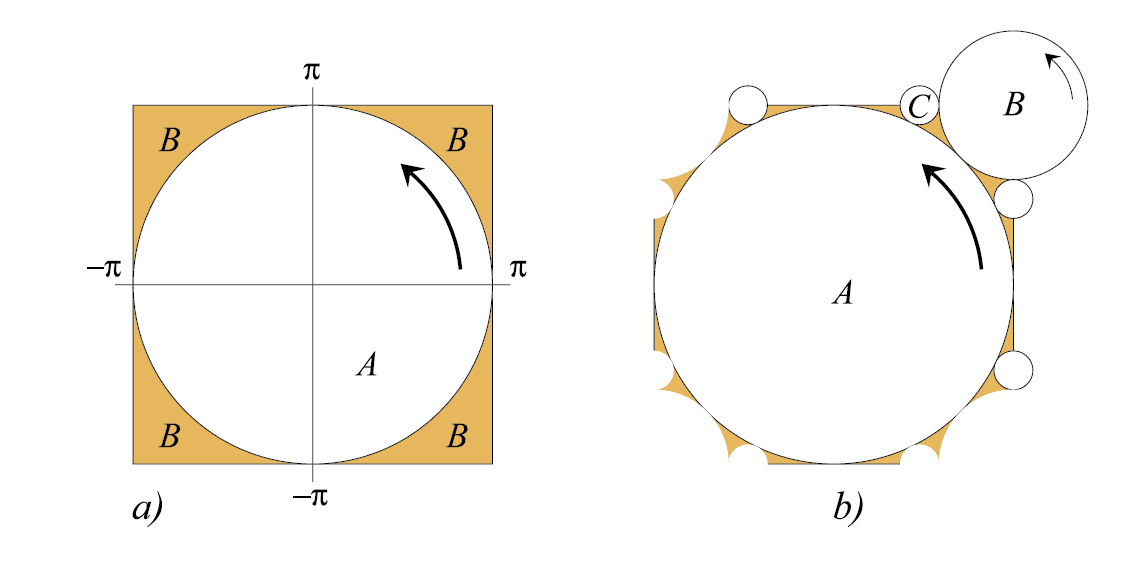
\includegraphics{images/img_18_1.PNG}
		Повороты в зоне Бриллюэна прямоугольной решетки. \mathbf{a} Мы можем ограничиться областью внутри самого большого круга, который вписывается в зону Бриллюэна (A). Затененной областью (B) пренебрегают и амплитуда там заменяется на ноль. Это хорошо, если сильно флуктуирующие моды в пространстве $\vec x$ можно игнорировать, например, на фотографии с прямоугольной сеткой пикселей. \mathbf{b} Унитарность восстанавливается, если мы также заполняем оставшуюся часть зоны Бриллюэна также кружками, B, C и т.д., чем больше, тем лучше (как объяснено в тексте), но никогда не перекрываются. На рисунке заштрихованные области также должны быть заполнены кружками. Оператор вращения должен вращать каждый круг на один угол (стрелки)
}
		\caption{
		\label{i18.1} }
	\end {center}
\end {figure}



Мы заполняем всю зону Бриллюэна круговыми областями, так что они полностью покрывают все пространство без перекрытий. Как будет объяснено вкратце, мы предпочитаем держать эти круги как можно больше, чтобы получить наилучший\footnote{“Лучший " здесь означает, что эффект вращения максимально локальный, как будет видно в дальнейшем.} результат. Действие оператора вращения теперь будет определено как соответствующее вращению на один и тот же угол $\varphi$ внутри всех этих окружностей (стрелки на фиг. \ref{i18.1} a и b). Под "кругами" мы здесь подразумеваем круговые области, или, если $d>2, $ области, ограниченные $(d-1)$-сферами.

Это-почти-лучшее\footnote{Небольшое осложнение, которое можно вылечить, объясняется вскоре после эквалайзера. (\ref{18.19})}, что мы можем сделать в зоне Бриллюэна, будучи пространством векторов Фурье $\vec{\kappa}$ . Причина, по которой мы разделяем зоны Бриллюэна на идеально сферические области, а не на другие формы, становится ясной, если мы исследуем действие этого оператора в $\vec{x}$-пространстве: как этот оператор работает в исходном пространстве сайтов решетки $\vec{x}$?

Давайте сначала рассмотрим действие одного круга, в то время как данные по остальной части зоны Бриллюэна заменяются нулем. Сначала возьмем круг (если $d=2$ ) или сферу (если $d=3$), центр которой находится в начале координат, а ее радиус равен $r .$ Проецирование этого круга означает, что в $\vec{x}$ -пространстве волновая функция $\psi (\vec{x})$ размазывается следующим образом:

\begin{equation}\label{18.13}
	\begin{aligned}
\psi^{\prime}(\vec{x}) &=(2 \pi)^{-d} \sum_{\vec{x}^{\prime}} \int_{|\vec{k}|<r} \mathrm{d}^{d} \vec{\kappa} e^{i \vec{k} \cdot\left(\vec{x}-\vec{x}^{\prime}\right)} \psi\left(\vec{x}^{\prime}\right) \\
&=\sum_{\vec{x}^{\prime}}\left(\frac{r}{\pi}\right)^{d} K_{d}\left(\frac{r}{\pi}\left|\vec{x}-\vec{x}^{\prime}\right|\right) \psi\left(\vec{x}^{\prime}\right)
\end{aligned}
\end{equation}


Ядром этого вращательно симметричного выражения оказывается функция Бесселя:

\begin{equation}\label{18.14}
	K_{d}(y)=\frac{\pi^{\frac{d-1}{2}}}{2^{d} \Gamma\left(\frac{d+1}{2}\right)} \int_{-1}^{1} \mathrm{d} k\left(1-k^{2}\right)^{\frac{d-1}{2}} e^{i \pi k y}=(2 y)^{-d / 2} J_{d / 2}(\pi y)
\end{equation}

\begin{figure}[ht]
	\begin{center}
		\scalebox{0.4}{
		   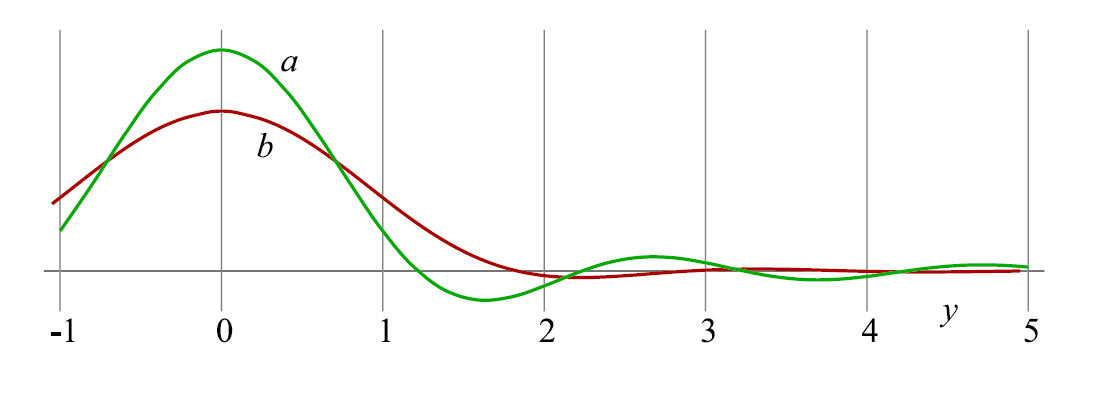
\includegraphics{images/img_18_2.png}
		}
		\caption{
		\label{i18.2}  The function $K_d (y)$, \mathbb{a} for $d = 2$, and \mathbb{b} for $d = 5$}
	\end {center}
\end {figure}

Это гладкая функция, падающая на бесконечность в виде степени $y$ (см. \ref{i18.2}):

\begin{equation}\label{18.15}
	K_{d}(y) \longrightarrow \frac{2 \sin \pi\left(y+\frac{1-d}{4}\right)}{\pi(2 y)^{\frac{d+1}{2}}} \quad \text { as } y \rightarrow \infty
\end{equation}


Мы делаем вывод из эквалайзера. (\ref{18.13}) что, проецируя внутреннюю часть окружности с радиусом $r$ в зону Бриллюэна, подразумевает размазывание данных на решетке по нескольким узлам решетки во всех направлениях, используя ядро $K_{d}(y)$. Чем меньше радиус $r,$ тем дальше размазывание, поэтому мы должны стараться держать наши круги (сферы) как можно больше.

Далее мы заметим, что большинство кругов на рис. \ref{i18.1} смещены от центра. Смещение вектора $\vec{\kappa}_{1}$ в зоне Бриллюэна соответствует умножению в конфигурационном пространстве на экспоненту $e^{i \vec{k}_{1} \cdot \vec{x}}$. Проецирование окружности с радиусом $r$ и ее началом на пятно $\vec{\kappa}_{1}$ в зоне Бриллюэна означает деление волновой функции $\psi(\vec{x})$ на экспоненту $e^{i \vec{k}_{1} \cdot \vec{x}},$ размазывание ее ядром $K_{d}(y)$, затем умножение с показателем снова (таким образом, мы приводим окружность к началу координат, проецируем ее на начало координат).централизованный круг, затем переместите его обратно туда, где он был). Это равносильно смазыванию исходной волновой функции модифицированным ядром

\begin{equation}\label{18.16}
	K_{d}\left(y, \vec{\kappa}_{1}\right)=K_{d}(y) e^{i \vec{\kappa}_{1} \cdot\left(\vec{x}-\vec{x}^{\prime}\right)}, \quad y=\frac{r}{\pi}\left|\vec{x}-\vec{x}^{\prime}\right|
\end{equation}


Если мы сложим проекции всех окружностей, которыми мы покрыли зону Бриллюэна, то общий эффект будет таким, что мы восстановим исходную волновую функцию на решетке. И теперь мы можем вращаться. Вращение круга $\left (r, \kappa_{1}\right)$ в зоне Бриллюэна на любой угол $\varphi$ имеет точно такой же эффект , как (1) нахождение размазанной волновой функции с помощью ядра $K_{d}(y) e^{-i \vec{k}_{1} \cdot \vec{x}^{\prime}},$ вращение результирующей непрерывной функции на угол $\varphi$ in $\vec{x}$- пространство, а затем умножение с экспоненциальной $e^{i \vec{k}_{1} \cdot \vec{x}}$. Если мы сложим вместе эффекты всех кругов, то получим оператор вращения. Если мы хотим получить эффект ортогонального вращения $\Omega$ в $\vec{x}$ - пространство, то это приводит к


\begin{equation}\label{18.17}
	\psi^{\prime}(\vec{x})=\sum_{\vec{x}^{\prime}} \sum_{i} K_{d}\left(\frac{r_{i}}{\pi}\left|\Omega \vec{x}-\vec{x}^{\prime}\right|\right) e^{i \vec{k}_{i} \cdot\left(\vec{x}-\vec{x}^{\prime}\right)} \psi\left(\vec{x}^{\prime}\right)
\end{equation}

где индекс $i$ отсчитывает круги, покрывающие зону Бриллюэна.

Преобразования, описанные в этом подразделе, образуют вполне приемлемую группу вращений, сходящуюся к обычным вращениям в пределе континуума. Это можно легко увидеть, заметив, что в континуальном случае преобладают малые значения $\vec{\kappa}$, которые все находятся в первичном круге. Другие круги также вращают волновые функции в нужное место, но они движутся только вдоль быстро колеблющихся частей, в то время как векторы $\vec{\kappa}_{1}$ остаются ориентированными в исходном направлении.

Искомые групповые свойства этого оператора вытекают из того факта, что окружности охватывают зону Бриллюэна ровно один раз.

\begin{equation}\label{18.18}
	\Omega_{3}=\Omega_{1} \Omega_{2}
\end{equation}


Конечно, операция (\ref{18.17}), называемая $R(\Omega)$, - это не совсем обычное вращение. Если $T (\vec{a})$ - это перевод над нерешеточным вектором $\vec{a}$ , как описано в разделе \ref{ch18.2.1} тогда

\begin{equation}\label{18.19}
	R(\Omega) T(\vec{a}) \neq T(\Omega \vec{a}) R(\Omega)
\end{equation}


и более того, если $\Omega$ выбран одним из элементов кристаллической группы решетки, $R (\Omega)$ все равно не совпадает с самим $\Omega$. Этот последний дефект можно вылечить, но мы не будем вдаваться в эти подробности.

Лучшая особенность этого оператора вращения заключается в том, что он, по-видимому, действует действительно локально в $\vec{x}$ - пространстве, лишь слегка распространяя точки решетки с ядрами функций Бесселя \ref{18.14}, но у него также есть недостатки: будет чрезвычайно трудно построить какой-то детерминированный закон эволюции, который уважает это преобразование как симметрию. По этой причине мы теперь рассмотрим другие рецепты непрерывного преобразования, которые дают вращения.


\subsubsection{Непрерывные вращения 2: использование зарядов Нётер и дискретной подгруппы}\label{ch18.2.3}

В детерминированной теории мы хотим определить закон эволюции, который учитывает наши симметрии. Это требует другого выбора для определения задействованных симметрий. Для этого мы вводим теорему Нётер, как она была введена в начале этой главы. Например, симметрия при сдвигах во времени связана с сохранением энергии, симметрия сдвига связана с сохранением импульса, а симметрия вращения приводит к сохранению момента импульса. Относимся к этим консервативным количествам в качестве нетеровых зарядов. Все эти консервативные заряды являются наблюдаемыми величинами, и поэтому, если мы хотим исследовать их в квантовой теории, которую мы относим к детерминированной системе, тогда эта детерминированная система должна также демонстрировать наблюдаемые величины, которые могут быть непосредственно связаны с зарядами Нетера.

В формализме $PQ$ в некотором смысле заложены нетеровские платежи за трансляционную симметрию. Переводы в переменные $Q_i$ связаны с величинами $p_i$, целые части которых $P_i$ являются онтологическими наблюдаемыми. Генерируют только дробные части
трансляции, которые тогда должны быть целочисленными шагами на решетке Q. Нам нужны обе составляющие импульса. Если длина решетки мала, кванты целочисленных частей импульсов велики. У планет очень большие импульсы, у холодных атомов очень маленькие импульсы. Большие импульсы также являются источниками гравитационных полей, и как таковые непосредственно наблюдаемые. Как насчет региона с переходной экономикой? Это происходит в очень знакомой области - единица импульса Планка составляет $\approx 6,5$ кгм / с. Импульс в этой области должен быть смесью наблюдаемых $P$ и операторов смещения $Q$, тогда как в обычной физике мы не замечаем ничего особенного в этой области.

В случае углового момента мы можем заметить, что угловой момент все равно квантуется. Можем ли мы связать онтологически наблюдаемую (возможную) момент импульса? Не так легко, потому что момент импульса состоит из некоммутирующих компонентов. В лучшем случае мы будем иметь онтологические квантованные переменные, играющие роль «классических частей» углового момента, дополненных квантовыми степенями свободы (переменными), которые восстанавливают правила коммутации. Мы наблюдаем, что для малых частиц угловой момент наблюдается лишь частично; иногда это уметь, иногда изменчиво. Для больших систем угловой момент наблюдается с некоторой погрешностью.

Это приводит нас к рассмотрению следующей структуры - и в действительности нам придется использовать аналогичные методы всякий раз, когда группа симметрии становится большой, то есть она имеет очень много элементов. Поскольку угловые импульсы не являются коммутативными, они не могут быть достаточно онтологическими, но их «классические части» должны быть. Поэтому предположим, что операторы полных угловых моментов $J_i$ можно записать следующим образом:


\begin{equation}\label{18.20}
	Ji = Li + ^ i, [Ji, Jj ^ = iSijkJk
\end{equation}

где $L_i$ представляет ожидаемые значения $J_i$ во всех онтологических состояниях, так что $L_i$ являются beables. A представляет остаток, и его ожидаемые значения в онтологических состояниях исчезают:

\begin{equation}\label{18.21}
	
\end{equation}

В следующем подразделе будет показана явная процедура получения $L_i$ и A ,.

\subsubsection{Непрерывные вращения 3: использование операторов действительных чисел p и q, построенных из P и Q}\label{ch18.2.4}

Если наша теория определена на решетке, есть еще один отличный способ восстановить многие симметрии случая континуума, используя трюк $PQ$, как он был раскрыт в разд. 16. Мы увидели эту теорию струн, раздел 17.3, был переписан таким образом, что строка перемещается по решетке в целевом пространстве, где решетка в основном описывает целые части координат, в то время как пространство между узлами решетки фактически соответствует собственным состояниям операторов смещения для переменные импульса P. Вместе они образуют континуум, и, поскольку вся система эквивалентна теории струн континуума, она также разделяет все симметрии непрерывного перемещения и вращения с этой теорией.

Позволяя применять этот механизм, теория струн оказывается более мощной, чем теории точечных частиц; правила коммутации операторов в целевом пространстве принципиально отличаются, и теория струн позволяет целевому пространству быть в большом числе измерений.

Таким образом, в формализме $P Q$ мы теперь используем континуальное определение углового момента. Рассмотрим волновую функцию одной частицы в трех пространственных измерениях, так что она живет на произведении трех $P, Q$ решеток. Эти решетки порождают три квантовые координаты $q_{i} .$ Его гильбертово пространство $\mathcal{H}$ является пространством произведения трех Гильбертовых пространств $\mathcal{H}_{1}, \mathcal{H}_{2}$ и $\mathcal{H}_{3}$
Пишите, как в Эквалайзерах. ( 16.18) и (16.19)

\begin{equation}\label{}
	
\end{equation}

$$
q_{i}^{\mathrm{op}}=Q_{i}+a_{i}^{\mathrm{op}}, \quad p_{i}^{\mathrm{op}}=2 \pi P_{i}+b_{i}^{\mathrm{op}}
$$

so that the angular momentum operator is (in the 3 -dimensional case)

\begin{equation}\label{}
	
\end{equation}

$$
J_{i}=\varepsilon_{i j k} q_{j}^{\mathrm{op}} p_{k}^{\mathrm{op}}=\varepsilon_{i j k}\left(2 \pi Q_{j} P_{k}+2 \pi a_{j}^{\mathrm{op}} P_{k}+Q_{j} b_{k}^{\mathrm{op}}+a_{j}^{\mathrm{op}} b_{k}^{\mathrm{op}}\right)
$$

since the expectation values of $\left.a_{i}^{\mathrm{op}} \text { and } b_{i}^{\mathrm{op}} \text { vanish in the ontological states, lont }\right\rangle=$

$|\vec{P}, \vec{Q}\rangle,$ and since the last term will be $\leq \mathcal{O}(2 \pi),$ we can identify $L_{i}$ with the first term:

\begin{equation}\label{}
	
\end{equation}

$$
L_{i} \approx 2 \pi \varepsilon_{i j k} Q_{j} P_{k}
$$

Note, that the $L_{i}$ are quantized in multiples of $2 \pi$ rather than one, as one might have expected, so Eq. ( 18.24) cannot hold exactly.

Let us now inspect the modifications on the commutation rules of these angular momentum operators caused by the edge states. In each of the three Hilbert spaces $\mathcal{H}_{i}, i=1,2,3,$ we have Eq. $(16.22),$ while the operators of one of these Hilbert spaces commute with those of the others. Writing the indices explicitly:

\begin{equation}\label{}
	
\end{equation}


$\left[q_{1}, p_{1}\right]=i \mathbb{I}_{2} \mathbb{I}_{3}\left(\mathbb{I}_{1}-\left|\psi_{e}^{1}\right\rangle\left\langle\psi_{e}^{1}\right|\right), \quad\left[q_{1}, p_{2}\right]=0, \quad$ and cyclic permutations
$$
(18.25)
$$

where $\mathbb{I}_{i}$ are the identity operators in the $i$ th Hilbert space, and $\left|\psi_{e}^{i}\right\rangle$ are the edge states on the $i$ th $P, Q$ lattice. One then easily derives that the three angular momentum operators $J_{i}$ defined in the usual way, Eq. $(18.23),$ obey the commutation rules

\begin{equation}\label{}
	
\end{equation}

$\left[J_{1}, J_{2}\right]=i J_{3} \mathbb{I}_{1} \mathbb{I}_{2}\left(\mathbb{I}_{3}-\left|\psi_{e}^{3}\right\rangle\left\langle\psi_{e}^{3}\right|\right), \quad$ and cyclic permutations. $\quad(18.26)$


The importance of this result is that now we observe that the operator $J_{3}$ only acts in Hilbert spaces 1 and $2,$ but is proportional to the identity in $\mathcal{H}_{3}$ (since $J_{3}$ contains only $q_{1}, q_{2}, p_{1},$ and $p_{2}$ ). So the projection operator for the edge state $\left|\psi_{e}^{3}\right\rangle$ commutes with $J_{3} .$ This implies that, if we limit ourselves to states that are orthogonal to the edge states, they will also rotate to states orthogonal to the edge states. In this subspace of Hilbert space the rotations act normally. And we think that this is remarkable, because certainly the "ontological" basis defined on the six-dimensional
$\vec{P}, \vec{Q}$ lattice has no built-in continuous rotation invariance at all.


\subsubsection{Квантовые симметрии и классическая эволюция}\label{ch18.2.5}

In previous subsections it was observed that, when we project classical models on Hilbert spaces, new symmetries may emerge. These are symmetry transformations that map classical states onto superpositions of states. A few examples were shown. None of our procedures are fool proof. In the special case to be discussed next, we study time translation invariance. As stated earlier, we might split the energy
$E$ into a classical part $(\delta E)$ and a quantum part (the generator of discrete time translations, the Hamiltonian $H$ that lies in the interval $[0,2 \pi / \delta t) .$ However, this would suggest that we can only measure energies with $2 \pi / \delta t$ as our margin of error. That cannot be right: if $\delta t$ is the Planck time, then the energy quantum is the Planck energy, $E_{\text {Planck }},$ which is about 543 kiloWatt-hours; yet we pay our electricity bills per kiloWatt-hour, and those bills are certainly ontological. Mutations in our DNA profiles might require only a couple of electron Volts to take place, and these might be crucial for our genetically inherited identities; an electron Volt is about $10^{-28}$ times the Planck energy. Even that may have to be (mostly) ontological.

Of course we are primarily interested in symmetries that are symmetries of the evolution operator. The cogwheel model, Sect. $2.2 .1,$ for instance has the classical symmetry of rotations over $N$ steps, if $N$ is the number of cogwheel position states. But if we go to the energy eigenstates $|k\rangle_{H}, k=0, \ldots N-1(\text { Eqs. }(2.21) \text { and }(2.22))$ we see that, there, a translation over $n$ teeth corresponds to multiplication of these states as follows:

\begin{equation}\label{}
	
\end{equation}

$$
|k\rangle_{H} \rightarrow e^{2 \pi i k n / N}|k\rangle_{H}
$$

since these are eigenstates of the Hamiltonian, this multiplication commutes with
$H$ and hence the symmetry is preserved by the evolution law. We now found out that we can enlarge the symmetry group by choosing the multiplication factors in frequency space

\begin{equation}\label{}
	
\end{equation}


$$
|k\rangle_{H} \rightarrow e^{2 \pi i k \alpha / N}|k\rangle_{H}
$$

where $\alpha$ now may be any real number, and this also corresponds to a translation in time over the real number $\alpha .$ This enhances the symmetry group from the group of the cyclic permutations of $N$ elements to the group of the continuous rotations of a circle.

\subsubsection{Квантовые симметрии и классическая эволюция 2}\label{ch18.2.6}

Другой довольно тривиальный, но интересный пример симметрии, который расширяется, если мы применяем наши квантовые конструкции, встречается в простом клеточном автомате в любом числе d пространственных измерений. Рассмотрим булевы переменные u (x, t) = ± 1, распределенные по всем четным узлам в пространстве-времени решетки, то есть по всем точкам (x, t) = (x1, ..., xd, t) с xi и t все целые числа и x1 + + xd +1 = четные.

Let the evolution law be

\begin{equation}\label{}
	
\end{equation}

$$
\sigma(\vec{x}, t+1)=\left(\prod_{i=1}^{d} \sigma\left(\vec{x}+\vec{e}_{i}, t\right) \sigma\left(\vec{x}-\vec{e}_{i}, t\right)\right) \sigma(\vec{x}, t-1)
$$

where $\vec{e}_{i}$ are the unit vectors in the $i$ th direction in $d$ dimensional space. Or: the product of the data on all direct space-time neighbours of any odd site $(\vec{x}, t)$ is
$+1 .$ This law is manifestly invariant under time reversal, and we see that it fixes all variables if the data are given on a Cauchy surface consisting of two consecutive layers in time $t, t-1 .$ The classical model has the manifest translation symmetry over vectors $\delta x=\left(a_{1}, \ldots, a_{d}, \tau\right)$ with $\sum_{i} a_{i}+\tau$ even.

Now let us introduce Hilbert space, and consider the odd lattice sites. On these odd sites, we define the action of changeables $\sigma_{1}\left(\vec{x}_{1}, t_{1}\right)$ as follows:
The data on the time frame $t=t_{1},$ are kept unchanged; on the time frame $t=t_{1}-1,$ only $\sigma\left(\vec{x}_{1}, t_{1}-1\right)$ changes sign, and all others remain unchanged; consequently, according to the evolution law, also on the frame $t=t_{1}+1$ only $\sigma\left(\vec{x}_{1}, t_{1}+1\right)$ changes sign, all others stay the same.
The reason for the notation $\sigma_{1}$ is that in a basis of Hilbert space where $\sigma\left(\vec{x}_{1}, t_{1}-1\right)=\sigma_{3}=\left(\begin{array}{c}{ 1}&{0} \\ {0} & {-1}\end{array}\right),$ our new operator is $\sigma_{1}\left(\vec{x}, t_{1}\right)=\sigma_{1}=\left(\begin{array}{cc}{0} & {1} \\ {1} & {0}\end{array}\right),$ as in
the Pauli matrices. Now, checking how the action of $\sigma_{1}(\vec{x}, t)$ propagates through the lattice, we observe that

\begin{equation}\label{}
	
\end{equation}

$$
\sigma_{1}(\vec{x}, t+1)=\left(\prod_{i=1}^{d} \sigma_{1}\left(\vec{x}+\vec{e}_{i}, t\right) \sigma_{1}\left(\vec{x}-\vec{e}_{i}, t\right)\right) \sigma_{1}(\vec{x}, t-1)
$$

where now the vector $(\vec{x}, t)$ is even, while in Eq. ( 18.29) they were odd. Thus the product of the changeables $\sigma_{1}\left(\vec{x}^{\prime}, t^{\prime}\right)$ that are direct space-time neighbours of an even site $(\vec{x}, t)$ is also one. since we recovered the same evolution law but now on the sites that before were empty, our translation symmetry group now has twice as many elements. Now, we can perform a translation over a vector, whose sum of components is odd, but the states in Hilbert space then have to undergo a transformation; at every site:

\begin{equation}\label{}
	
\end{equation}

$$
|\psi(\vec{x}, t)\rangle \rightarrow U_{\mathrm{op}}|\psi(\vec{x}, t)\rangle, \quad U_{\mathrm{op}} \sigma_{1} U_{\mathrm{op}}^{-1}=\sigma_{3} ; \quad U_{\mathrm{op}}=\frac{1}{\sqrt{2}}\left(\begin{array}{rr}
{1} & {1} \\
{1} & {-1}
\end{array}\right)
$$

since $U^{2}=1,$ this is actually a reflection. This means that the succession of two odd translations gives an even translation without further phase changes.

This simple model shows how the introduction of Hilbert space may enhance the symmetry properties of a theory. In this case it also implies that the Brillouin zone for momentum space becomes twice as large (see Fig. 18.3 ). A quantum physicist living in this world will not be able to distinguish the even sites from the odd ones.


\subsection{Большие группы симметрии в CAI}\label{ch18.3}

Мы заканчиваем эту главу общим видом больших групп симметрии, таких как трансляции в пространстве и во времени, и группы Лоренца. У них есть бесконечное количество групповых элементов. Теперь мы представляем, что наши модели автоматов имеют дискретное количество информации, распределенной в пространстве и времени. Как мы можем иметь на них бесконечные и / или непрерывные группы симметрии?
Наше впечатление от предыдущих результатов состоит в том, что обычные генераторы симметрии, используемые в квантовых теориях, будут операторами, которые всегда состоят из комбинаций вероятностей и переменных: нетеровские заряды, такие как момент импульса, энергия и импульс, будут иметь классические ограничения, которые совершенно заметны, следовательно, они являются beables; но квантово-механически операторы не коммутируют, и поэтому должны быть заменяемые части.
Любимые части будут сопряжены с мельчайшими операциями симметрии, такими как очень маленькие сдвиги и повороты. Они вряд ли будут полезны в качестве подлинных преобразований в онтологических данных - конечно, нет, так как они должны коммутировать с beables.
Изменяемые части этих операторов не являются онтологическими наблюдаемыми, поскольку они не коммутируют. Формализм PQ, разработанный в разд. 16, является реализацией этой концепции расщепления операторов: здесь, как в пространстве позиций, так и в пространстве импульсов, целочисленные части операторов трансляции являются beables, дробные части являются переменными. Поп операторы непрерывного перевода состоят из обоих ингредиентов. Мы подозреваем, что это должно стать общей чертой всех больших групп симметрии, в частности самого гамильтониана, и это то, что мы попытаемся реализовать в следующей главе 19.



\begin{equation}\label{18.}
	
\end{equation}

\begin{equation}\label{18.}
	
\end{equation}

\begin{equation}\label{18.}
	
\end{equation}

\begin{equation}\label{18.}
	
\end{equation}

\begin{equation}\label{18.}
	
\end{equation}

\begin{equation}\label{18.}
	
\end{equation}

\begin{equation}\label{18.}
	
\end{equation}

\begin{equation}\label{18.}
	
\end{equation}

\begin{equation}\label{18.}
	
\end{equation}

\begin{equation}\label{18.}
	
\end{equation}

\begin{equation}\label{18.}
	
\end{equation}

\begin{equation}\label{18.}
	
\end{equation}

\begin{equation}\label{18.}
	
\end{equation}

\begin{equation}\label{18.}
	
\end{equation}








\end{document}

